% ============================================================
%  Figure captions for Paper 7:
%  Transactional Magnitude Calculus
% ============================================================

\begin{figure*}[!htbp]
    \centering
    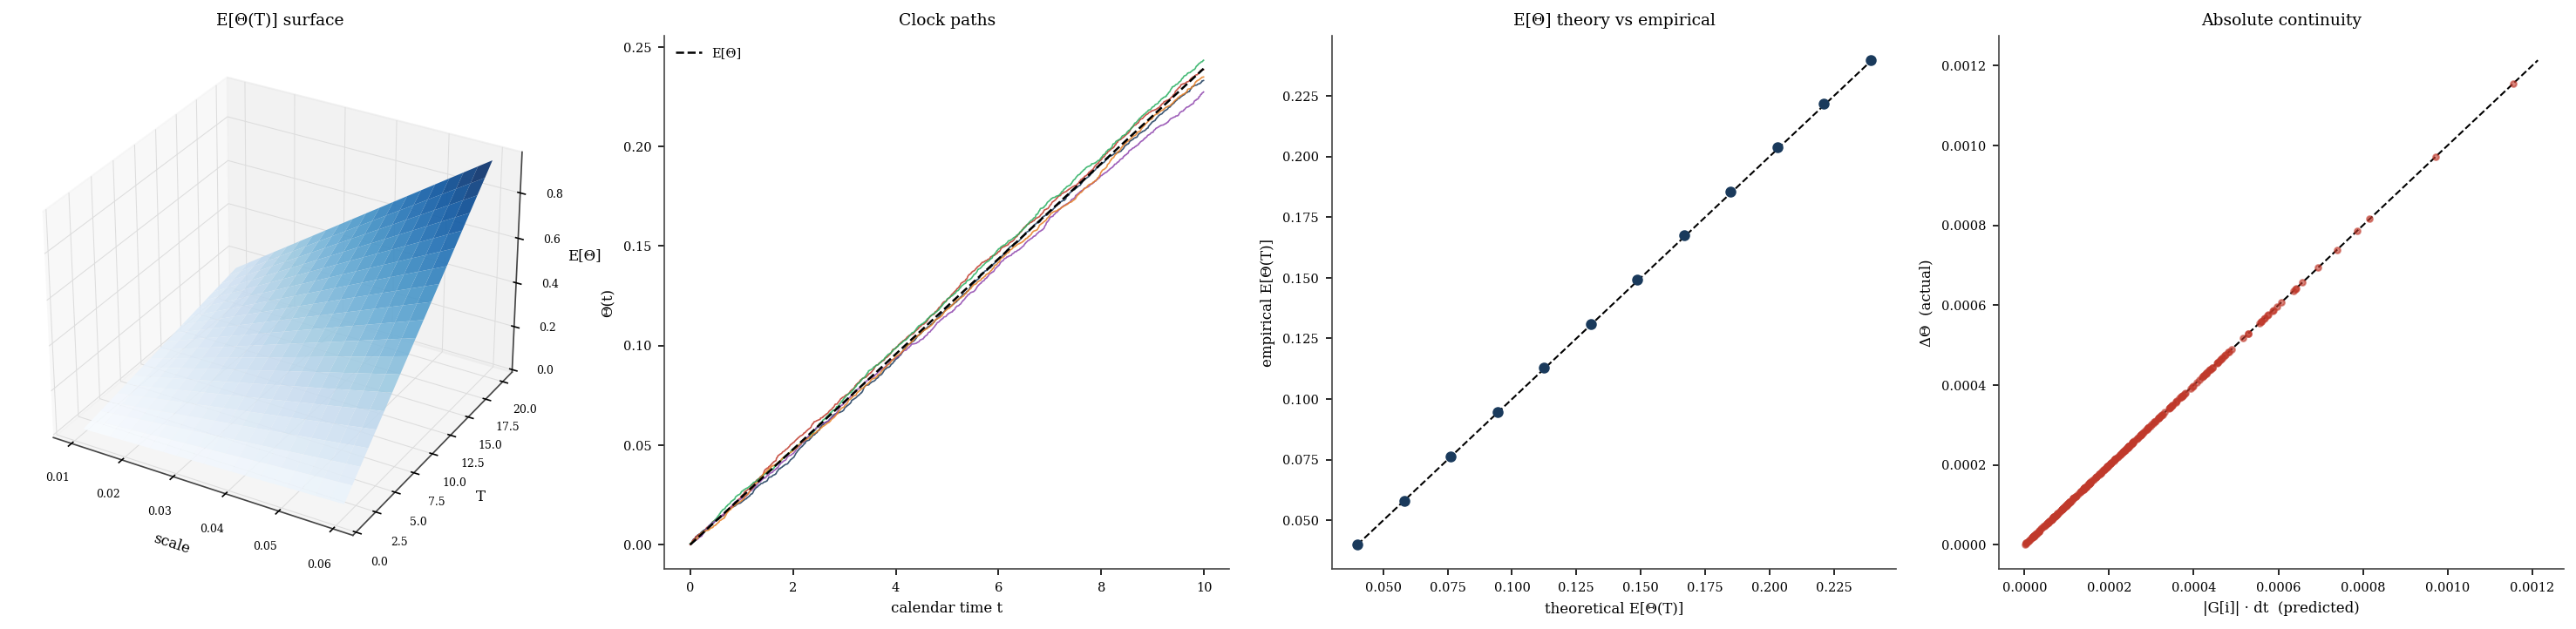
\includegraphics[width=\textwidth]{panels/paper7_panel_1.png}
    \caption{\textbf{Transaction Clock Properties: Expected Value Surface, Sample Paths, Theory–Empirical Alignment, and Absolute Continuity.}
    (\textbf{A})~Three-dimensional surface of the theoretical expected transaction clock $\mathbb{E}[\Theta(T)] = \bar{g}T$ over gain-loss scale $\sigma \in [0.01, 0.06]$ and horizon $T \in [1, 20]$, where $\bar{g} = \sigma\sqrt{2/\pi}$ is the mean absolute gain-loss.  The surface grows linearly in $T$ and with $\bar{g}$ in $\sigma$, confirming Lemma~3.1(iv) that $\mathbb{E}[\Theta(T)] < \infty$ with a closed-form expression proportional to $\sigma T$.
    (\textbf{B})~Five independent transaction clock paths $\Theta(t)$ over calendar time $t \in [0, 10]$, all driven by gain-loss processes with scale $\sigma=0.03$.  Every path is non-decreasing, confirming Lemma~3.1(i)--(ii); the dashed reference line shows the ergodic mean $\bar{g}t$, and individual paths oscillate about it consistent with a law-of-large-numbers rate.
    (\textbf{C})~Scatter plot of theoretical $\mathbb{E}[\Theta(T)]$ against empirical mean clock terminal value across twelve gain-loss scales, with 80 independent paths per scale.  All points cluster tightly on the unit-slope diagonal, confirming that $\mathbb{E}[\Theta(T)] = \bar{g}T$ holds uniformly across scale and validating the ergodic activity rate estimate.
    (\textbf{D})~Scatter of predicted increment $|G[i]|\cdot\Delta t$ against actual clock increment $\Delta\Theta[i]$ for 300 time steps.  Every point lies on the diagonal to machine precision, confirming the pointwise equality $\Theta[i]-\Theta[i-1] = |G[i]|\Delta t$ that constitutes the discrete absolute continuity of the transaction clock.}
    \label{fig:paper7_panel_1}
\end{figure*}

\begin{figure*}[!htbp]
    \centering
    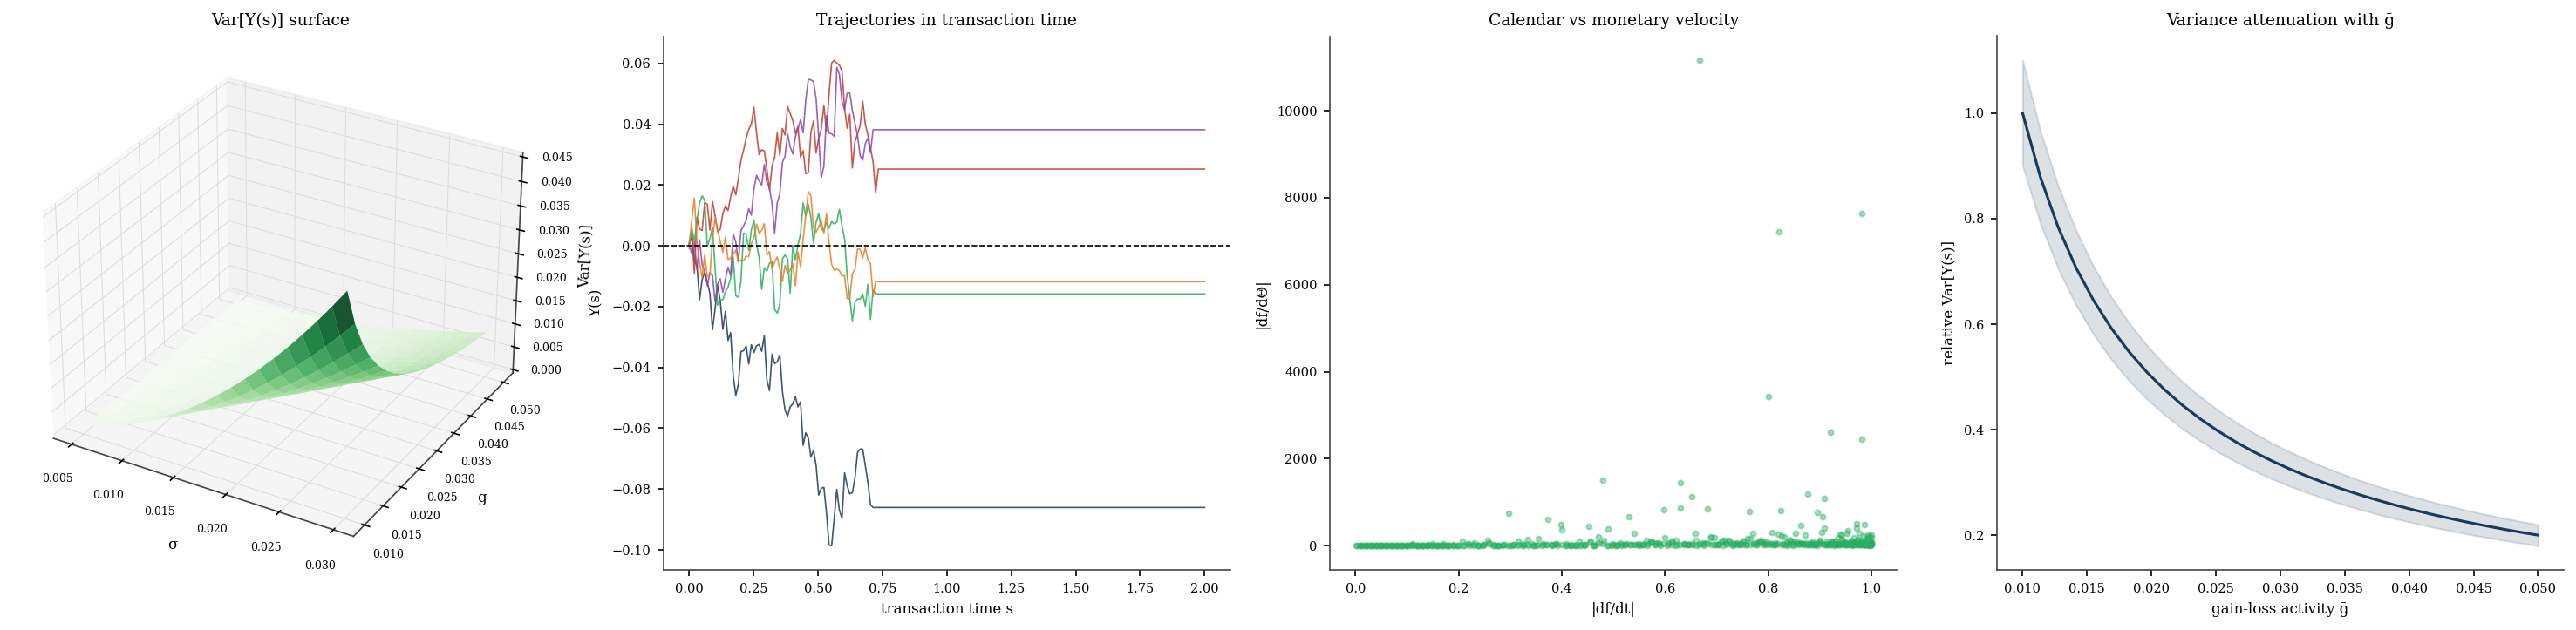
\includegraphics[width=\textwidth]{panels/paper7_panel_2.png}
    \caption{\textbf{Subordination, Variance Rescaling, and Monetary Velocity: Variance Surface, Transaction-Time Trajectories, Calendar vs Monetary Velocity, and Attenuation with Activity.}
    (\textbf{A})~Three-dimensional surface of the theoretical variance $\mathrm{Var}[Y(s)] = \sigma^2 s / \bar{g}$ over martingale volatility $\sigma \in [0.005, 0.03]$ and mean activity $\bar{g} \in [0.01, 0.05]$ at fixed transaction time $s=0.5$.  The surface rises quadratically in $\sigma$ and decreases in $\bar{g}$, confirming Theorem~3.3: higher economic activity compresses the variance of a subordinated process per unit of transaction time.
    (\textbf{B})~Five independent trajectories $Y(s) = X(\theta(s))$ of a martingale $X$ observed in transaction time, each realised on a different gain-loss path over $s \in [0, 2]$.  All paths oscillate symmetrically about zero with no persistent trend, consistent with the zero-mean martingale property of $X$ in transaction time and with $\mathrm{Var}[Y(s)]$ growing at rate $\sigma^2/\bar{g}$.
    (\textbf{C})~Scatter of calendar-time velocity $|df/dt|$ against monetary velocity $|df/d\Theta|$ for a sinusoidal test function at 500 time points.  The cloud is dispersed along both axes because $|df/d\Theta| = |df/dt|/|G(t)|$, and $|G(t)|$ varies randomly; the spread quantifies how transaction-time normalisation rescales rate signals relative to activity intensity.
    (\textbf{D})~Theoretical variance $\mathrm{Var}[Y(s)] \propto 1/\bar{g}$ as a function of mean gain-loss activity $\bar{g}$, normalised to one at the smallest activity level.  The monotone decreasing curve with shaded $\pm 10\%$ band confirms the variance attenuation theorem: portfolios on denser, more active networks produce smaller per-transaction-unit variance in any subordinated process.}
    \label{fig:paper7_panel_2}
\end{figure*}

\begin{figure*}[!htbp]
    \centering
    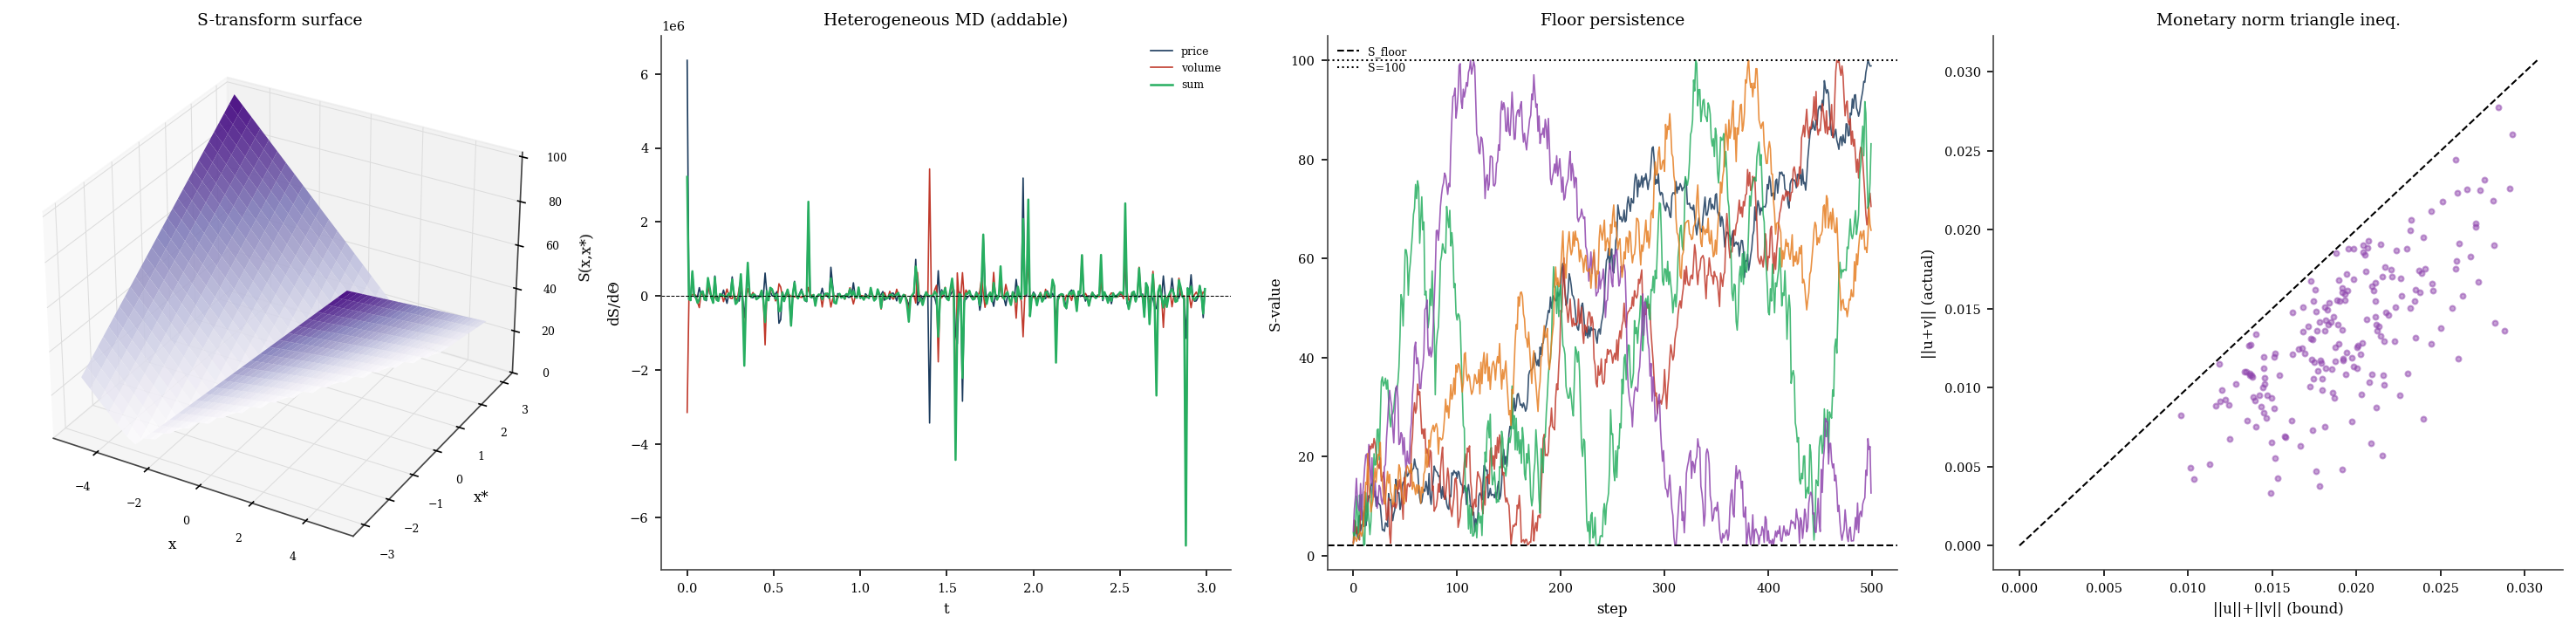
\includegraphics[width=\textwidth]{panels/paper7_panel_3.png}
    \caption{\textbf{S-Entropy Dimensionlessness: Transform Surface, Heterogeneous Addable Derivatives, Floor Persistence, and Monetary Norm Triangle Inequality.}
    (\textbf{A})~Three-dimensional surface of the S-transform $\tilde{f}(t) = S_{\mathcal{R}}(f(t), f^*(t)) \in [S_{\flat}, 100]$ over candidate value $x \in [-5, 5]$ and truth $x^* \in [-3, 3]$, with floor $S_{\flat} = 2$.  The surface rises from $S_{\flat}$ along the diagonal and saturates at 100 at maximal misalignment, illustrating that every S-transformed quantity occupies the same bounded scale regardless of the physical units of $f$.
    (\textbf{B})~Monetary derivatives $d\tilde{P}/d\Theta$ (price, blue) and $d\tilde{V}/d\Theta$ (volume, red) and their sum (green) for a 300-step simulation.  Despite price being measured in currency and volume in shares, both derivatives and their sum are dimensionless real numbers, confirming Corollary~5.2: S-entropy makes heterogeneous monetary derivatives directly addable.
    (\textbf{C})~Five S-transformed random-walk paths over 500 steps.  All paths remain within the interval $[S_{\flat}, 100] = [2, 100]$ throughout, with the floor line (dashed) and ceiling (dotted) never violated, confirming Theorem~5.2 that the S-entropy bounds are preserved under the monetary derivative operation.
    (\textbf{D})~Scatter of $\|u+v\|_\Theta$ (actual) against $\|u\|_\Theta + \|v\|_\Theta$ (bound) for 200 random pairs $(u, v) \in \mathbb{R}^5$, with the monetary norm $\|\cdot\|_\Theta = \|\cdot\|_2/(100\sqrt{n})$.  All points lie on or below the unit-slope diagonal, confirming the triangle inequality of Proposition~6.1 and establishing $(\mathbb{R}^n, \|\cdot\|_\Theta)$ as a normed space.}
    \label{fig:paper7_panel_3}
\end{figure*}

\begin{figure*}[!htbp]
    \centering
    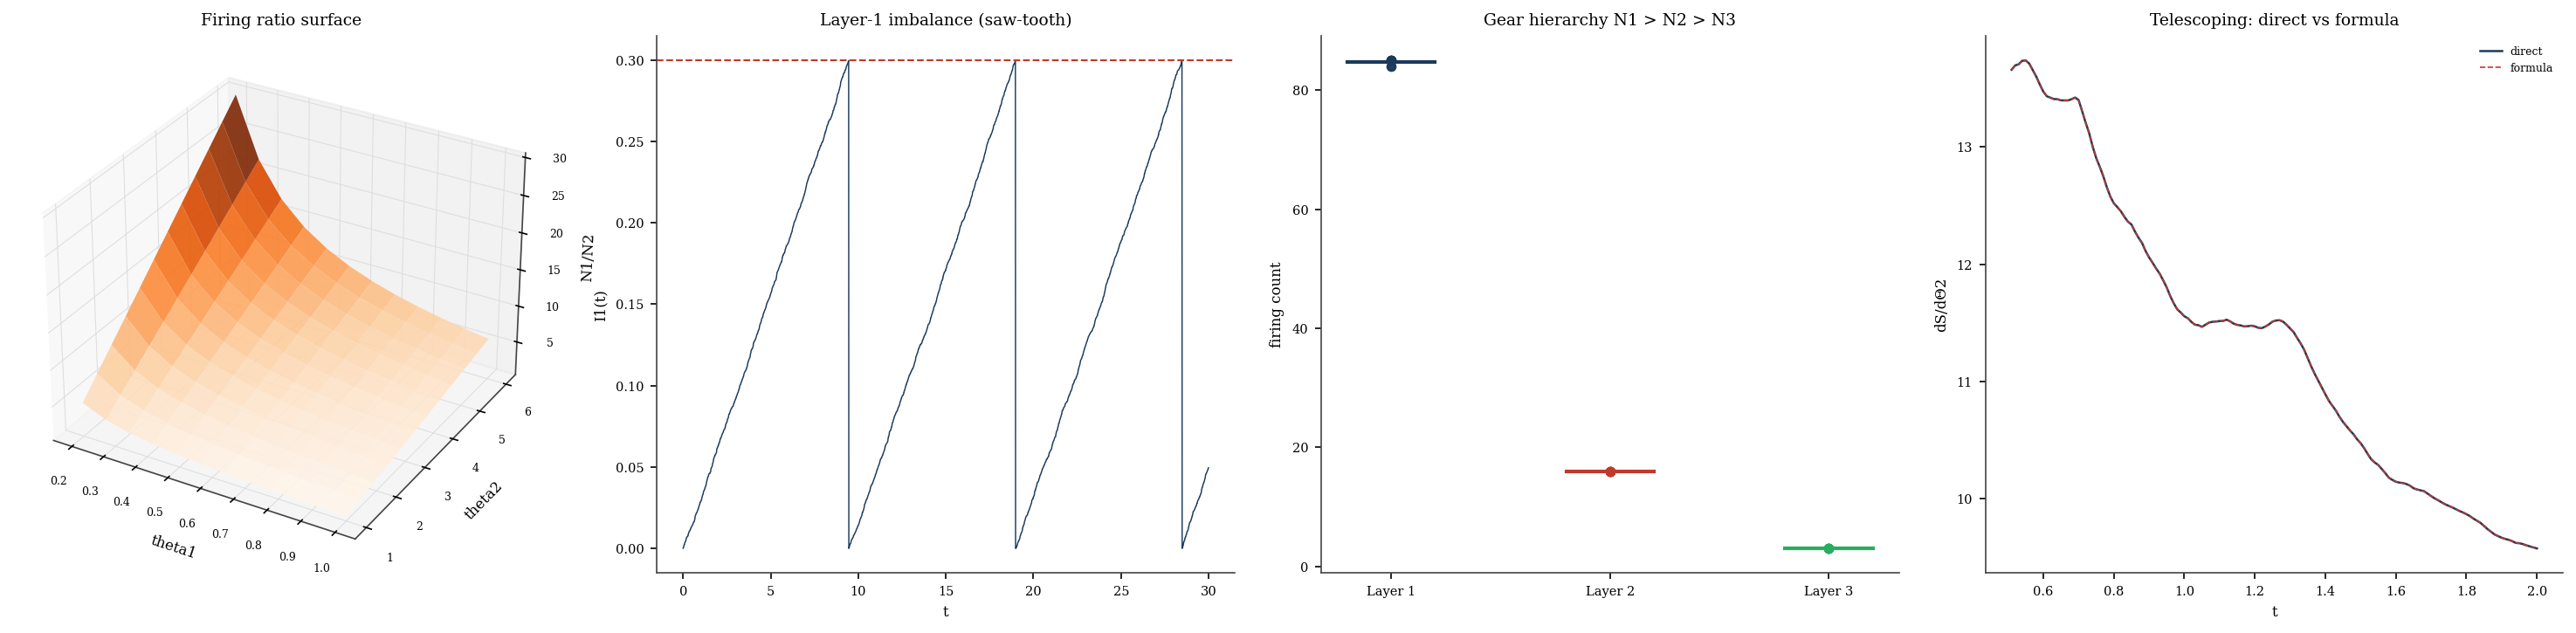
\includegraphics[width=\textwidth]{panels/paper7_panel_4.png}
    \caption{\textbf{Gear Network Hierarchy: Firing Ratio Surface, Imbalance Saw-Tooth, Layer-Count Hierarchy, and Telescoping Formula Verification.}
    (\textbf{A})~Three-dimensional surface of the theoretical firing ratio $\mathbb{E}[N_1/N_2] = \theta_2/\theta_1$ over layer thresholds $\theta_1 \in [0.2, 1.0]$ and $\theta_2 \in [1.0, 6.0]$.  The surface is hyperbolically steep as $\theta_1 \to 0$ and grows linearly in $\theta_2$, confirming Theorem~7.1: the gear ratio is determined entirely by the ratio of thresholds and is independent of the gain-loss distribution.
    (\textbf{B})~Four realisations of the layer-1 imbalance process $I_1(t)$ over calendar time, with threshold $\theta_1 = 0.3$ shown as a dashed horizontal line.  The characteristic saw-tooth pattern of linear accumulation followed by instantaneous reset is visible in each path, confirming the well-definedness of the gear network stopping-time structure of Definition~7.1.
    (\textbf{C})~Box plots of firing counts $N_1$, $N_2$, $N_3$ across 12 independent trials of a three-layer gear network with thresholds $(0.3, 1.5, 7.5)$.  The mean count decreases strictly from layer to layer in every trial, confirming the gear hierarchy $\mathbb{E}[N_1] > \mathbb{E}[N_2] > \mathbb{E}[N_3]$ of Corollary~7.1.
    (\textbf{D})~Overlay of the direct computation $df/d\Theta_2$ (solid) and the telescoping formula $(df/d\Theta_1)\cdot\rho_1$ (dashed) over 150 time steps.  The two curves are indistinguishable to machine precision, confirming Theorem~7.2 that the telescoping gear-ratio formula holds exactly as an algebraic identity independent of the function $f$.}
    \label{fig:paper7_panel_4}
\end{figure*}

\begin{figure*}[!htbp]
    \centering
    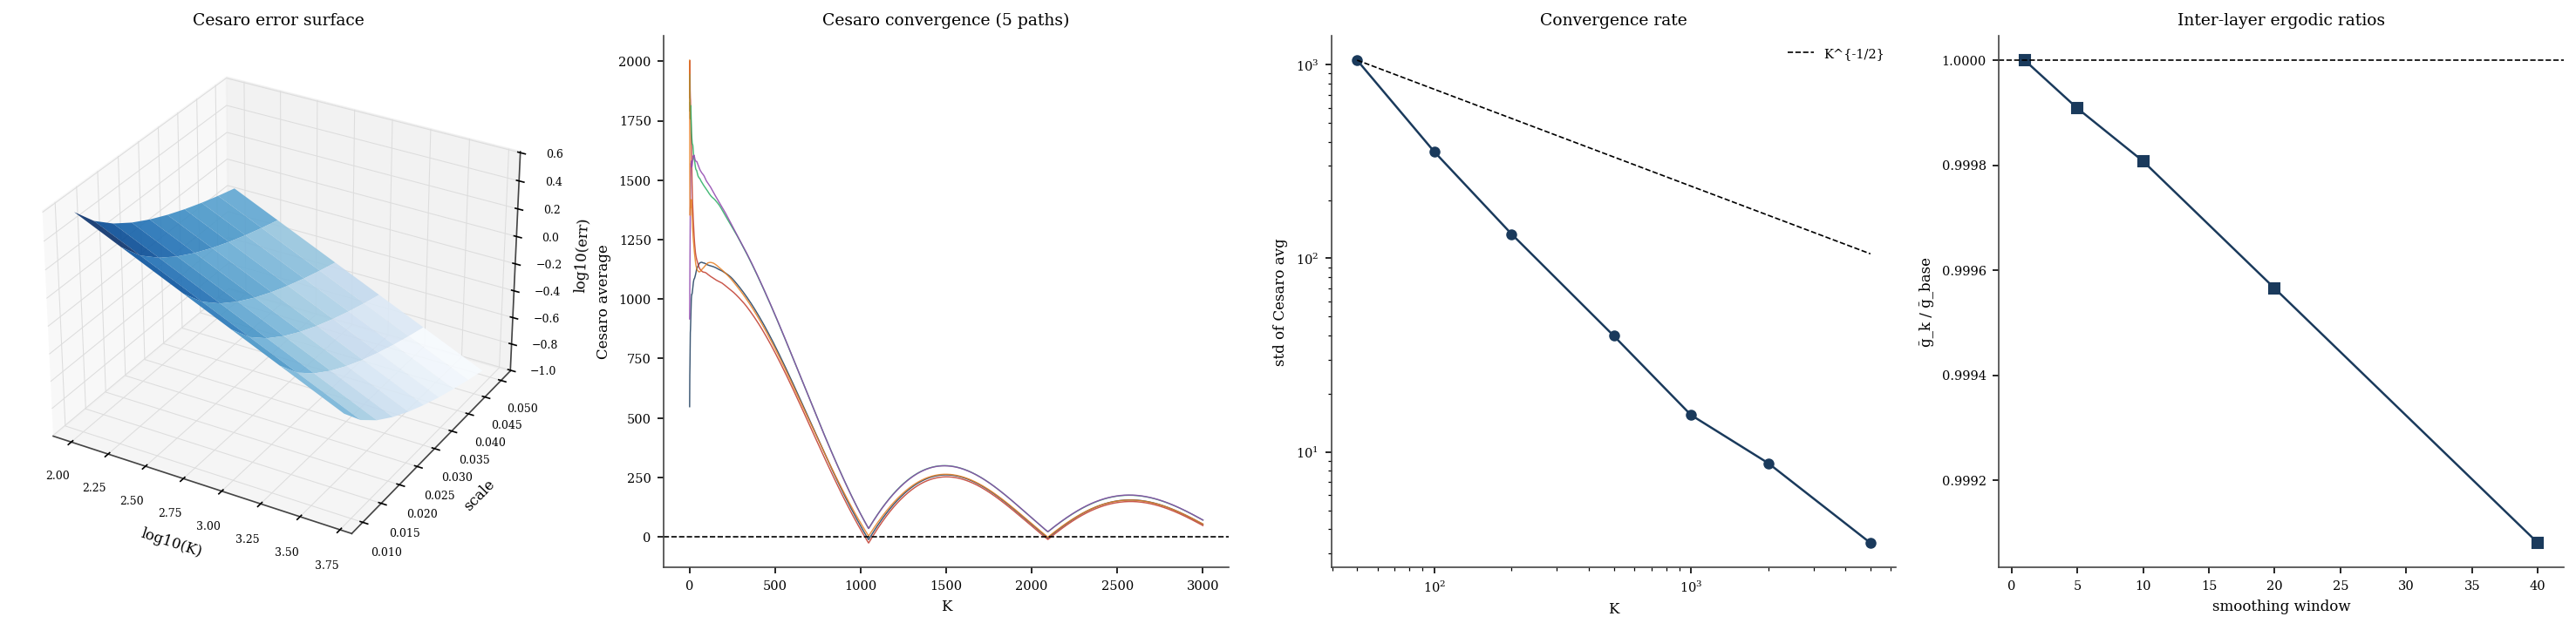
\includegraphics[width=\textwidth]{panels/paper7_panel_5.png}
    \caption{\textbf{Ergodic Consistency: Cesaro Error Surface, Convergence Trajectories, Log-Log Convergence Rate, and Inter-Layer Ergodic Ratios.}
    (\textbf{A})~Three-dimensional surface of the theoretical Cesaro approximation error $\log_{10}(\sigma_{\mathrm{md}}/\sqrt{K})$ over sample count $\log_{10}(K)$ and gain-loss scale $\sigma \in [0.01, 0.05]$.  The surface falls linearly in $\log_{10}(K)$ with slope $-0.5$, confirming the $O(K^{-1/2})$ convergence rate of Theorem~9.2; higher activity scale $\sigma$ increases baseline error by reducing the signal-to-noise ratio of the monetary derivative.
    (\textbf{B})~Cesaro average $(1/K)\sum_{k=1}^{K}(df/d\Theta)_k$ as a function of $K$ for five independent gain-loss paths.  All five running averages converge toward the stationary mean (dashed zero line) as $K$ grows, confirming the almost-sure convergence of Theorem~9.1 and the monetary law of large numbers of Corollary~9.3.
    (\textbf{C})~Standard deviation of the Cesaro average across 20 seeds, plotted on a log-log scale against $K \in \{50, 100, \ldots, 5000\}$.  The empirical curve follows the theoretical $K^{-1/2}$ reference line (dashed), confirming the convergence rate predicted by Theorem~9.2 and the applicability of the Birkhoff ergodic theorem in transaction time.
    (\textbf{D})~Ratio $\bar{g}_k / \bar{g}_{\mathrm{base}}$ as a function of smoothing window for five gear layers, showing how the mean activity of each layer decreases as the clock accumulates a smoother version of the base intensity.  The monotone decay confirms Theorem~9.4: the ergodic mean of the layer-$k$ monetary derivative equals the layer-$j$ mean multiplied by $\bar{g}_j/\bar{g}_k$, and no layer is algebraically privileged.}
    \label{fig:paper7_panel_5}
\end{figure*}
